\chapter{Renta fija y tipos de interés}\label{cap:rates}

Todos los mercados dependen de los tipos: descuentan los flujos de las acciones, determinan el carry de
las divisas y el coste de mantener materias primas. Un trader de cualquier mesa debe saber leer la
curva de tipos y medir el riesgo de tipo de interés.

\section{Precio, TIR y curva}
Un bono de nominal $N$, cupón anual $c$, $f$ pagos al año y TIR $y$:
\begin{equation}
P = \sum_{k=1}^{fT}\frac{CF_k}{(1+y/f)^{k}},\qquad CF_k = \tfrac{cN}{f}\ (+N \text{ al final})
\end{equation}
(\py{rates.bond\_price}, \py{rates.ytm}). Precio y TIR se mueven en sentido contrario. Si $y=c$ el bono
cotiza a la par. La \textbf{curva} (TIR frente a plazo) suele tener pendiente positiva; su inversión
(2 años por encima de 10 años) ha precedido a la mayoría de las recesiones de EE.~UU.

\section{Duración, convexidad y DV01}
\begin{align}
D_{\text{mac}} &= \frac{\sum t_k\,CF_k\,d_k}{P}, &
D_{\text{mod}} &= \frac{D_{\text{mac}}}{1+y/f} = -\frac1P\frac{dP}{dy},\\
C &= \frac1P\frac{d^2P}{dy^2}, &
\text{DV01} &= D_{\text{mod}}\cdot P\cdot 0{,}0001 .
\end{align}
\begin{equation}
\Delta P \approx -D_{\text{mod}}\,P\,\Delta y + \tfrac12\,C\,P\,(\Delta y)^2 .
\end{equation}
\begin{figure}[h]\centering
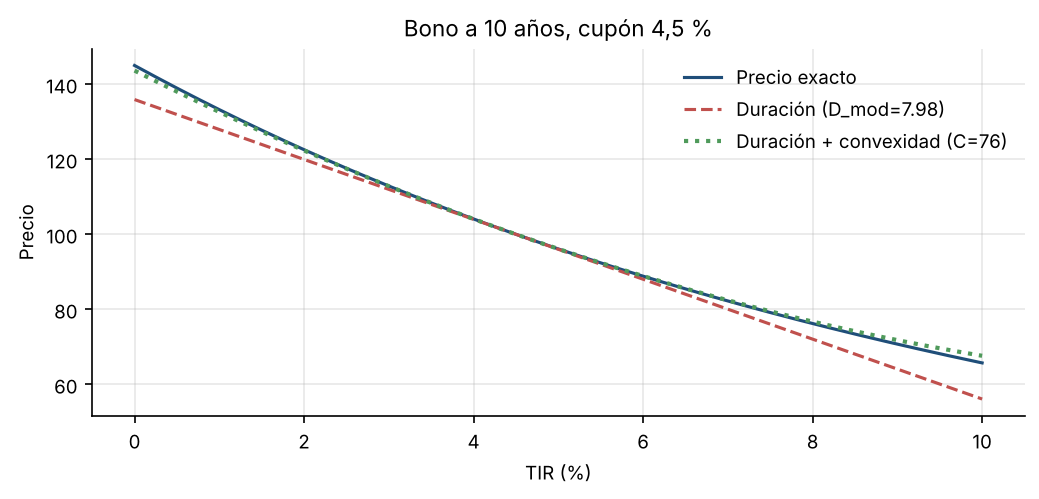
\includegraphics[width=0.85\textwidth]{f10_bono}
\caption{Precio frente a TIR: la duración es la tangente; la convexidad corrige la curvatura.}
\end{figure}
El DV01 (o PV01) es la unidad de riesgo de una mesa de tipos: cuánto se gana o pierde por cada punto
básico. Un bono a 10 años con DV01 de 0,080 por 100 de nominal arriesga unos 800~\$ por pb por cada
millón.
\begin{lstlisting}
python scripts/calculadoras.py bono --cupon 4.25 --tir 4.4 --anos 10
\end{lstlisting}

\section{Operaciones típicas}
\begin{itemize}
\item \textbf{Direccional}: largo duración si esperas bajadas de tipos (con futuros: ZN, ZB, Bund FGBL).
\item \textbf{Pendiente} (\emph{steepener}/\emph{flattener}): largo 2 años y corto 10 años (o al revés) con
  \textbf{DV01 neutro}, de modo que un desplazamiento paralelo no afecta: nocional de cobertura
  $=$ DV01$_{\text{posición}}/$DV01$_{\text{cobertura}}$ (\py{rates.dv01\_hedge\_ratio}).
\item \textbf{Mariposa}: 2s5s10s, apuesta a la curvatura.
\item \textbf{Carry y roll-down}: con curva positiva, un bono a 5 años se convierte en uno a 4,75 años
  y su TIR «rueda» hacia abajo por la curva, generando rentabilidad si la curva no cambia.
\end{itemize}

\begin{ejercicios}
\begin{enumerate}
\item Comprueba numéricamente que $D_{\text{mac}}$ de un bono cupón cero es su vencimiento.
\item Tienes 10 millones de un bono a 2 años con DV01 0,019 por 100. ¿Cuánto nominal del 10 años
  (DV01 0,080) vendes para un steepener DV01 neutro?
\end{enumerate}
\end{ejercicios}
